\documentclass{article}
\usepackage{cmap}
\usepackage[utf8]{inputenc}
\usepackage[english,ukrainian]{babel}
\usepackage{graphicx}
\usepackage{geometry}
\usepackage{listings}
\usepackage{float}
\geometry{
	a4paper,
	left=20mm,
	right=20mm,
	top=20mm,
	bottom=20mm
}
\lstset{
	language=c,
	tabsize=4,
	keepspaces,
	showstringspaces=false,
}
\graphicspath{ {./pictures} }
\setlength{\parindent}{4em}

\newcommand\subject{Алгоритми та структури даних}
\newcommand\lecturer{доцент кафедри ПЗ\\Коротєєва Т.О.}
\newcommand\teacher{асистент кафедри ПЗ\\Франко А.В.}
\newcommand\mygroup{ПЗ-22}
\newcommand\lab{5}
\newcommand\theme{Метод сортування злиттям}
\newcommand\purpose{Вивчити алгоритм сортування злиттям. Здійснити програмну реалізацію алгоритму сортування злиттям. Дослідити швидкодію алгоритму сортування злиттям}

\begin{document}
	\begin{normalsize}
		\begin{titlepage}
			\thispagestyle{empty}
			\begin{center}
				\textbf{МІНІСТЕРСТВО ОСВІТИ І НАУКИ УКРАЇНИ\\
					НАЦІОНАЛЬНИЙ УНІВЕРСИТЕТ "ЛЬВІВСЬКА ПОЛІТЕХНІКА"}
			\end{center}
			\begin{flushright}
				Інститут \textbf{КНІТ}\\
				Кафедра \textbf{ПЗ}
			\end{flushright}
			\vspace{200pt}
			\begin{center}
				\textbf{ЗВІТ}\\
				\vspace{10pt}
				До лабораторної роботи № \lab\\
				\textbf{На тему}: “\textit{\theme}”\\
				\textbf{З дисципліни}: “\subject”
			\end{center}
			\vspace{112pt}
			\begin{flushright}
				
				\textbf{Лектор}:\\
				\lecturer\\
				\vspace{28pt}
				\textbf{Виконав}:\\
				
				студент групи \mygroup\\
				Коваленко Д.М.\\
				\vspace{28pt}
				\textbf{Прийняв}:\\
				
				\teacher\\
				
				\vspace{28pt}
				«\rule{1cm}{0.15mm}» \rule{1.5cm}{0.15mm} 2022 р.\\
				$\sum$ = \rule{1cm}{0.15mm}……………\\
				
			\end{flushright}
			\vspace{\fill}
			\begin{center}
				\textbf{Львів — 2022}
			\end{center}
		\end{titlepage}
		
		\begin{description}
			\item[Тема.] \theme.
			\item[Мета.] \purpose.
		\end{description}
		
		\section*{Лабораторне завдання}
		Створити віконний проект та написати програму, яка реалізує алгоритм сортування Шелла.
		\begin{center}
			6. Задано одномірний масив дійсних чисел. До від’ємних елементів масиву застосувати функцію $sin(x)$. Отриманий масив посортувати в порядку спадання.
		\end{center}
		
		\section*{Теоретичні відомості}
	Сортування злиттям (англійською «Merge Sort») — алгоритм сортування, в основі якого лежить принцип «розділяй та володарюй» (англійською «Divide and Conquer»). В основі цього способу сортування лежить злиття двох упорядкованих ділянок масиву в одну впорядковану ділянку іншого масиву.
	
	Під час сортування в дві допоміжні черги з основної поміщаються перші дві відсортовані підпослідовності, які потім зливаються в одну і результат записується в тимчасову чергу. Потім з основної черги беруться наступні дві відсортовані підпослідовності і так до тих пір доки основна черга не стане порожньою. Після цього послідовність з тимчасової черги переміщається в основну чергу. І знову продовжується сортування злиттям двох відсортованих підпослідовностей. Сортування триватиме до тих пір поки довжина відсортованої підпослідовності не стане рівною довжині самої послідовності.
	
	Сортування злиттям можна задати рекурсивно: масив поділяється на дві приблизно рівні частини, які після сортування (тим самим способом) зливаються. Коли ж довжина частини масиву зменшується до 1, відбувається повернення з рекурсії. Завершуючи описання сортування злиттям, скажемо, що цей алгоритм є першим із ефективних алгоритмів сортування. У 1945 році його винайшов Джон фон Нейман, один із піонерів програмування.
	
	Час роботи алгоритму T(n) по впорядкуванню n елементів задовільняє рекурентному співвідношенню: $T(n) = 2\cdot T(\frac{1}{2}\cdot n) + O(n), деT(\frac{1}{2}\cdot n)$ - час на впорядкування половини масиву, $O(n)$ - час на злиття цих половинок.
		
		\subsection*{Покроковий опис роботи алгоритму сортування злиттям}
		\textbf{Алгоритм S - сортування злиттям}
		\begin{enumerate}  
			\item [\textbf{S1}] Ініціалізація індексів $i=1, j=1, k=1$.
			\item [\textbf{S2}] Виконувати $S3$-$S4$ доки $k<(n+m)$.
			\item [\textbf{S3}] Присвоїти змінні $i=1$, $j=n$.
			\item [\textbf{S4}] Якщо $xi  < yj$, то $zk = xi; i=i+1$, інакше $zk=yj, j=j+1$.
			\item [\textbf{S5}] $k=k+1$.
			\item [\textbf{S6}] Вихід.
		\end{enumerate}
		
		\newpage
		
		\section*{Хід роботи}
		\subsection*{Файл sort.rs}
		\begin{lstlisting}
use crate::data::Data;

pub fn sort(input: &mut [Data], res: &mut Vec<Vec<Data>>) {
	if input.len() < 2 {return;}
	
	let len = input.len();
	let mid = len / 2;
	sort(&mut input[..mid], res);
	sort(&mut input[mid..], res);
	
	let mut tmp = Vec::with_capacity(len);
	let mut i = 0;
	let mut j = mid;
	
	while i < mid && j < len {
		if input[i] < input[j] {
			tmp.push(input[i]);
			i += 1;
		} else {
			tmp.push(input[j]);
			j += 1;
		}
		res.push(tmp.to_vec());
	}
	if i < mid {
		tmp.extend_from_slice(&input[i..mid]);
	} else if j < len {
		tmp.extend_from_slice(&input[j..len]);
	}
	
	input.copy_from_slice(&tmp[..]);
}
\end{lstlisting}
		
		\section*{Результат роботи}
		\begin{figure}[H]
			\centering
			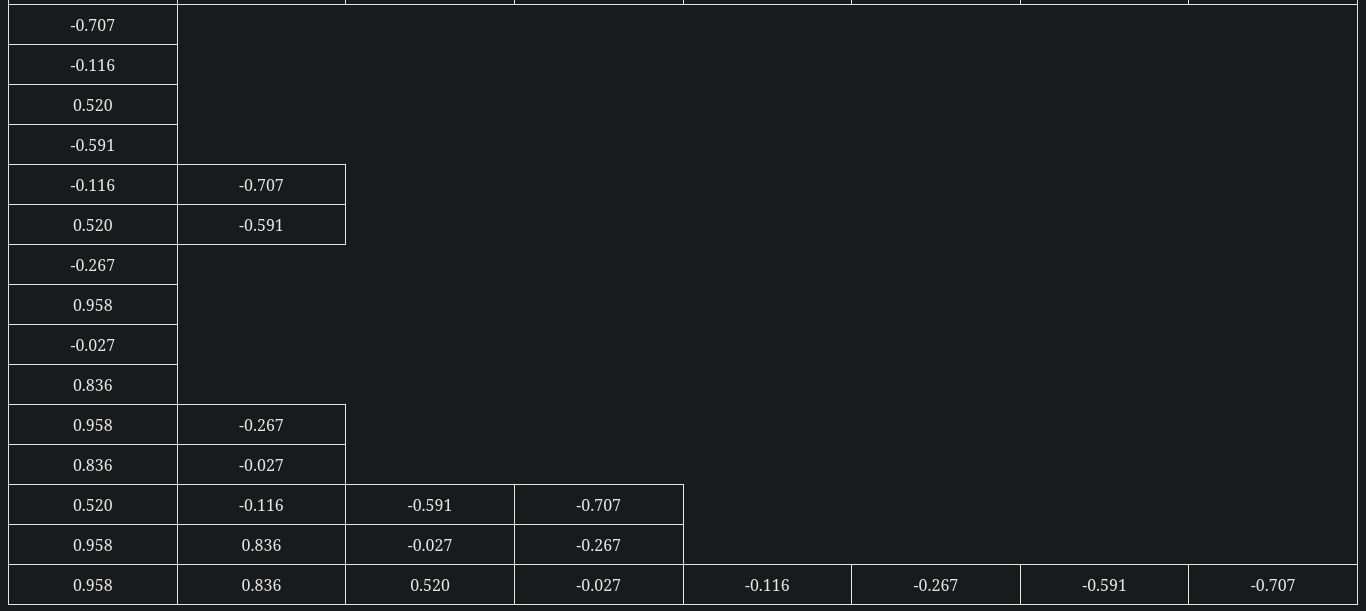
\includegraphics[scale=0.36]{1}
			\caption{Виконання програми}
		\end{figure}
		
		\section*{Висновок}
		Під час виконання лабораторної роботи я вивчив алгоритм сортування злиттям. Здійснив програмну реалізацію алгоритму сортування злиттям. Дослідив швидкодію алгоритму сортування злиттям.
		
	\end{normalsize}
\end{document}
